\chapter{Versuchsaufbau}

\section{Der Versuchsreaktor am WSA}
 
Der am WSA stehende Modell-Wirbelschichtreaktor (siehe Abb.1.1) besteht aus einem Ofen in dem der Reaktor eingelassen ist. Mit Hilfe des Ofens lassen sich im Reaktor Temperaturen von bis zu 1280�C erzielen. Der Reaktor (siehe Abb. \vref{fig:Abb1} ) hat einen Durchmesser von di=34 mm. Innerhalb des Reaktors befindet sich ein keramisches Beet bestehend aus $Al_2O_3$, welches der Erzeugung der Wirbelschicht dient. Dem Versuchsreaktor ist ein Schaltbrett vorgeschaltet. Auf dem Schaltbrett k�nnen verschiedene Gase beliebig vermischt werden, um eine gew�nschte Reaktion einstellen zu k�nnen. Im Fall der Pyrolyse wird dem Reaktor in aller Regel reiner Stickstoff zugef�hrt. Aber auch Kohlenstoffdioxid, Umgebungsluft, eine Kombination der Gase oder ein beliebiges anderes Gas k�nnen zus�tzlich angeschlossen werden. Das Abgas wird nach dem Reaktor �ber beheizte Schl�uche zun�chst in einen Filter, zur Abscheidung m�glicher Festk�rper, gleitet und darauf dem FTIR zugef�hrt, wo es auf seine Zusammensetzung untersucht werden kann. Der Reaktor wird in einem diskontinuierlichen Batch-Betrieb mit Brennstoff versorgt. In der Regel betragen die zugef�hrten Mengen Brennstoff zwischen 5 und 15 mg pro Probe.

\begin{figure}[htb]
	\centering
	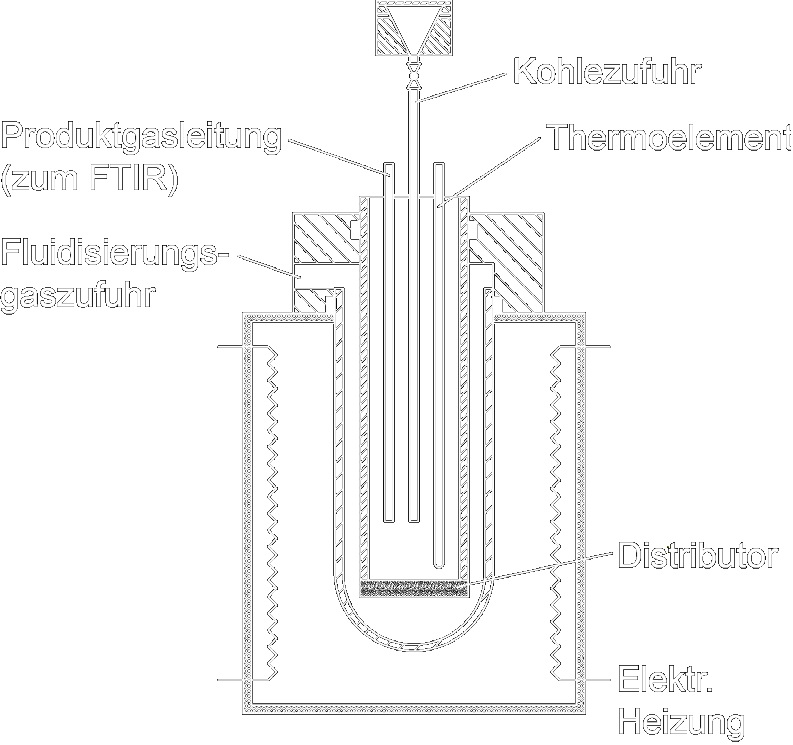
\includegraphics[scale=0.4]{bilder/Versuchsaufbau/Aufbau}
	\caption{Aufbau des Wirbelschichtreaktors}
	\label{fig:Abb1}
	
\end{figure}

\section{Funktionsweise des FTIR}

Zur Messung der Verbrennungsprodukte wird ein FTIR-Spektrometer eingesetzt. Ein FTIR-Spektrometer besteht grunds�tzlich aus zwei schwarzen K�rpern. Der eine dient als Strahlungsquelle zur Erzeugung einer Schwarzk�rperstrahlung, der andere als Strahlungsdetektor und misst die Energie der einfallenden Photonen. Zwischen der Strahlungsquelle und dem Strahlungsdetektor befinden sich noch teils bewegliche Spiegel um den Strahlengang zu f�hren. Dabei durchl�uft die Ausgesendete Strahlung das zugef�hrte Gas und wird von diesem Teilweise absorbiert. Aufgrund der Energie der Einfallenden Photonen kann geschlossen werden in welchen Wellenl�ngenbereichen Absorption vorliegt. Man kann auf diese Weise R�ckschl�sse �ber die Zusammensetzung des Gases ziehen, da jedes Gas �ber andere Absorptionseigenschafften verf�gt. So ist $CO_2$ beispielsweise als Treibhausgas bekannt, da gerade die W�rmestrahlung im Bereich von 4,17 $\mu$m bis 4,35 $\mu$m von $CO_2$ sehr stark absorbiert wird(siehe \vref{fig:Abb3}). Andere Gase absorbieren andere Wellenl�ngen und auch mit unterschiedlicher Intensit�t.

\begin{figure}[htb]
	\centering
	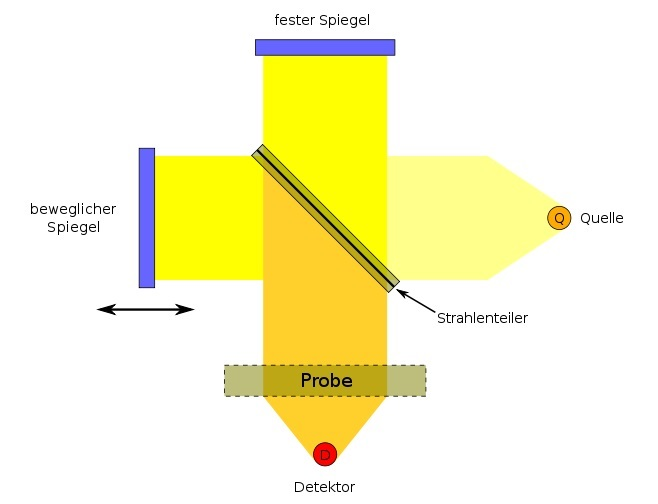
\includegraphics[scale=0.4]{bilder/Versuchsaufbau/658px-Ftir-spectrometer}
	\caption{Aufbau eines FTIR-Spektrometers}
	\label{fig:Abb2}
	
\end{figure}

\begin{figure}[htb]
	\centering
	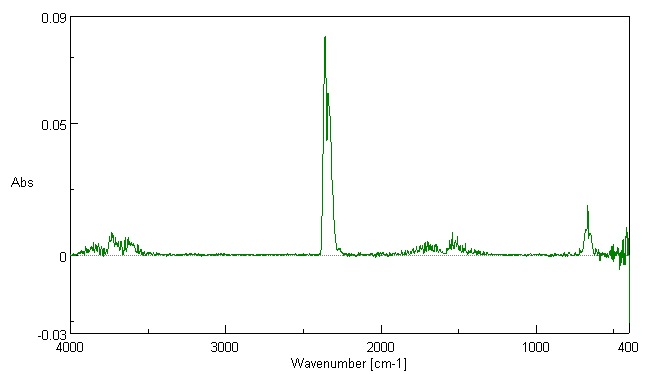
\includegraphics[scale=0.4]{bilder/Versuchsaufbau/CO2_ABS_FTIR_Dec_2012}
	\caption{Absorptionsspektrum von $CO_2$ in einem FTIR}
	\label{fig:Abb3}
	
\end{figure}
